\input SlidePreamble
\input preamble

\begin{document}

{\Huge

  \centerline{\bf TTIC 31230, Fundamentals of Deep Learning}
  \bigskip
  \centerline{David McAllester, Winter 2020}

  \vfill
  \centerline{\bf Representing Functions with Programs}
  \vfill
  \centerline{\bf Python, Assembler, and the Turing Tarpit}

  \vfill
  \vfill

\slide{Chomsky vs. Kolmogorov and Hinton}

\includegraphics[width=1.0 in]{\images/Chomsky} \begin{minipage}[b]{8in} Noam Chomsky: 
Natural language grammar cannot be learned by a universal learning algorithm.
This position is supported by the ``no free lunch theorem''.\end{minipage}

\vfill
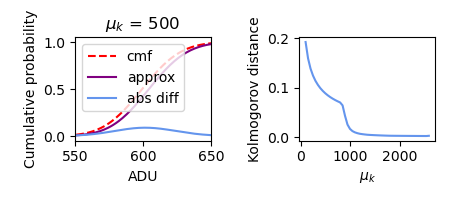
\includegraphics[height=1.0 in]{\images/Kolmogorov}
\includegraphics[height=1.0 in]{\images/Hinton}
\begin{minipage}[b]{7in}
Andrey Kolmogorov, Geoff Hinton: Universal learning algorithms exist. This position is supported by the ``free lunch theorem''.
\end{minipage}

\slide{The No Free Lunch Theorem}

\includegraphics[width=1.0 in]{\images/Chomsky} 

Without prior knowledge, such as universal grammar, it is impossible to make a prediction for an input you have not seen in the training data.


\vfill
{\bf Proof:} Select a predictor $h$ uniformly at random from all functions from ${\cal X}$ to ${\cal Y}$ and then take the data distribution to draw pairs $(x, h(x))$
where $x$ is drawn uniformly from ${\cal X}$.  No learning algorithm can predict $h(x)$ where $x$ does not occur in the training data.


\slide{The Occam Guarantee (Free Lunch Theorem)}

Consider a classifier $f$ written in C++ with an arbitrarily large standard library.

\vfill
Let $|f|$ be the number of bits needed to represent $f$.

\slide{The Occam Guarantee (Free Lunch Theorem)}

\vfill
$$0 \leq {\cal L}(h,x,y) \leq \lmax$$
\begin{eqnarray*}
{\cal L}(h)  & = &  E_{(x,y)\sim \mathrm{Pop}}\;{\cal L}(h,x,y) \\
\hat{{\cal L}}(h) & = & E_{(x,y)\sim \mathrm{Train}}\;{\cal L}(h,x,y)
\end{eqnarray*}

\vfill
Theorem: With probability at least $1-\delta$ over the draw of the training data the following holds simultaneously for all $f$.

{\color{red} $${\cal L}(f) \leq \frac{10}{9}\left(\hat{{\cal L}}(f) + \frac{5\lmax}{N_\mathrm{Train}}\left((\ln 2)|f| +\ln\frac{1}{\delta}\right)\right)$$}

\slide{Representing Functions with Programs}

Neural Turing Machines
Alex Graves, Greg Wayne, Ivo Danihelka, 2014

\vfill
(Actually a differentiable Von Neumann architecture)

\vfill
\centerline{\includegraphics[height = 3in]{../images/VNA}}

\vfill
The machine undergoes continuous state, discrete time, state transitions defined a differentiable feed-forward circuit.

\slidetwo{Compositional Attention Networks for Machine Reasoning}{Hudson and Manning, ICLR 2018}

\centerline{\includegraphics[height = 2.0in]{../images/MACcell}}

The MAC cell is similar to a gated RNN cell used as the decoder in translation.

\vfill
It is also similar to a Neural Turing Machine.

\vfill
It was applied to image-based question answering and uses attention over the image and the question during multi-step ``decoding''.

\slide{What about Python?}

High level scripting languages such as Python seem to be the most productive programming languages for human programmers.

\vfill
Does Python represent a particularly efective universal learning bias?

\vfill
Productivity in programming seems to be greatly enhanced by functional expressions (functional programming) and object-oriented programming
(objects, classes an inheretitance).

\vfill
This seems crucial if we want to somehow achieve I. J. Good's intelligence explosion.

\slide{The Turing Tarpit}

But in theory the choice of programming language does not matter.

\vfill
For any two Turing universal languages, say Python and Assmbler, there exists an interpreter $I$ for Python written in Assembler
where write $I(h)$ for the assember interpreter $I$ applied to Python program $h$.  We then get

$$|I(h)|_\mathrm{Assembler} = |h|_\mathrm{Python} + |I|_\mathrm{Assembler}$$

\vfill
Bootstrapping layers of language can make the interpreter small.


\slide{The Turing Tarpit}

$$|I(h)|_\mathrm{Assembler} = |h|_\mathrm{Python} + |I|_\mathrm{Assembler}$$

\vfill
Up to the additive constant of the interpreter, assembler gives just as good a learning bias as Python.

\vfill
Yet we know that the choice of language does matter --- Python is clearly better than assembler.


\slide{END}

}
\end{document}
